\section{Mischen von Serien- und Parallelschaltungen}
\subsection{Einleitung}
In elektronischen Schaltungen wird oft eine Kombination aus Reihen- und Parallelschaltungen verwendet, um spezifische elektrische Eigenschaften zu erreichen. Ziel dieses Versuchs ist es, die Teilströme und Spannungen in einer solchen Mischschaltung zu messen und mit den theoretisch berechneten Werten zu vergleichen. Dabei wird das Verhalten von Strom und Spannung an den Widerständen analysiert und die Funktionsweise der Schaltung umfassend untersucht.

\subsection{Theoretische Grundlagen}
Die Berechnung des Gesamtwiderstands \(R_{ges}\) und der Teilströme erfolgt nach den bekannten Gleichungen:

\paragraph{Reihenschaltung:}
\begin{equation}
    R_{ges} = R_1 + R_2 + \ldots + R_n
\end{equation}

\paragraph{Parallelschaltung:}
\begin{equation}
    \frac{1}{R_{ges}} = \frac{1}{R_1} + \frac{1}{R_2} + \ldots + \frac{1}{R_n}
\end{equation}

\paragraph{Teilströme in einer Parallelschaltung:}
Die Stromteilerregel wird verwendet, um die Teilströme \(I_1\) und \(I_2\) zu berechnen:
\begin{equation}
    \frac{I_k}{I_{ges}} = \frac{R_{gesamt}}{R_k}, \quad k = 1, 2
\end{equation}

\subsection{Versuchsaufbau}
Die untersuchte Schaltung besteht aus einer Kombination von zwei in Reihe geschalteten Widerständen (\(R_1, R_2\)) und zwei parallel geschalteten Widerständen (\(R_3, R_4\)), wie in Abbildung~\ref{fig:K3A1} dargestellt. Als Spannungsquelle wird eine Gleichspannung von \(U = 10 \,\unit{V}\) verwendet. Die Teilströme und Spannungen werden an definierten Messpunkten erfasst.

\begin{figure}[H]
    \centering
    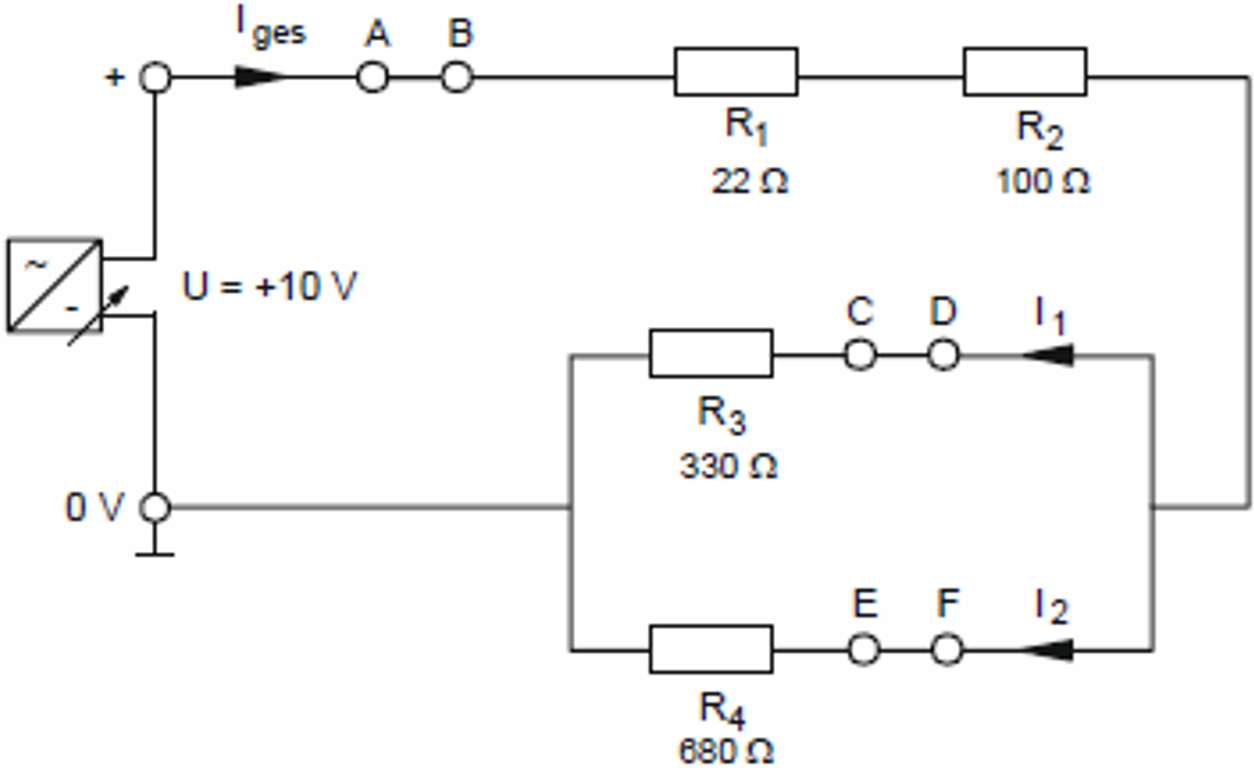
\includegraphics[width=0.6\textwidth]{Pictures/Kapitel3/Mischen von Reihen und Parallelschaltung.png}
    \caption{Schaltung zur Untersuchung des Stromflusses}
    \label{fig:K3A1}
\end{figure}

\subsection{Versuchsdurchführung}
Die Durchführung erfolgt in folgenden Schritten:
\begin{enumerate}
    \item Aufbau der Schaltung gemäß Abbildung~\ref{fig:K3A1}.
    \item Überprüfung der Versorgungsspannung \(U = 10 \, \unit{V}\) mit einem Multimeter.
    \item Messung der Teilströme an den Punkten A-B (\(I_{ges}\)), C-D (\(I_1\)) und E-F (\(I_2\)).
    \item Erfassung der Spannungen an den Widerständen \(R_1\), \(R_2\), \(R_3\) und \(R_4\).
    \item Vergleich der Messwerte mit den theoretischen Berechnungen.
\end{enumerate}

\subsection{Ergebnisse}
Die gemessenen und berechneten Werte sind in Tabelle~\ref{tab:K3T1} und Tabelle~\ref{tab:K3T2} zusammengefasst. Die theoretischen Werte werden mit den folgenden Gleichungen berechnet: 
\begin{align*}
    R_{ges} &= R_1 + R_2 + \frac{R_3 \cdot R_4}{R_3 + R_4}\\
    I_{ges} &= \frac{U}{R_{ges}}\\
    I_1 &= I_{ges} \cdot \frac{R_4}{R_3 + R_4}\\
    I_2 &= I_{ges} \cdot \frac{R_3}{R_3 + R_4}
\end{align*}

\begin{table}[H]
    \centering
    \caption{Gemessene und berechnete Ströme}
    \begin{tabular}{c c c c}
        \hline
        \multicolumn{4}{c}{Teilströme und Gesamtstrom/\unit{mA}}\\
        \hline
        \multicolumn{4}{c}{Messpunkte}\\
        \hline
       & A-B ($I_{ges}$) & C-D ($I_1$) & E-F ($I_2$)\\
        gemessen & 29,08 & 19,67 & 9,43\\
        berechnet & 29,05 & 19,56 & 9,49\\
        \hline     
    \end{tabular}
    \label{tab:K3T1}
\end{table}

\begin{table}[H]
    \centering
    \caption{Gemessene und berechnete Spannungen}
    \begin{tabular}{c c c c c}
         \hline 
         \multicolumn{5}{c}{Teilspannungen/\unit{V}} \\
         \hline
        & $U_{R1}$ & $U_{R2}$ & $U_{R3}$ & $U_{R4}$\\
        gemessen & 0,63 & 2,63 & 6,41 & 6,41\\
        berechnet & 0,64 & 2,90 & 6,50 & 6,50\\
         \hline
    \end{tabular}
    \label{tab:K3T2}
\end{table}

\subsection{Diskussion und Interpretation}
Die Messergebnisse stimmen gut mit den theoretischen Berechnungen überein. Kleine Abweichungen sind auf Messfehler oder Toleranzen der Widerstände zurückzuführen. Die Teilströme \(I_1\) und \(I_2\) folgen den Erwartungen der Stromteilerregel, während die gemessenen Spannungen die Eigenschaften der Reihen- und Parallelschaltungen bestätigen. Besonders hervorzuheben ist die hohe Übereinstimmung der Gesamtstrommessung \(I_{ges}\).

\paragraph{Abweichungen:}
\begin{itemize}
    \item \textbf{Widerstandstoleranzen:} Kleine Abweichungen in den nominellen Widerstandswerten könnten die Ergebnisse beeinflusst haben.
    \item \textbf{Messgeräte:} Die Genauigkeit der Multimeter beeinflusst die Messwerte geringfügig.
\end{itemize}

\newpage